\documentclass[11pt,a4paper]{article}
\usepackage[utf8]{inputenc}
\usepackage[T1]{fontenc}
\usepackage{geometry}
\usepackage{hyperref}
\usepackage{listings}
\usepackage{xcolor}
\usepackage{booktabs}
\usepackage{array}
\usepackage{fancyhdr}
\usepackage{enumitem}
\usepackage{float}
\usepackage{mdframed}
\usepackage{tikz}
\usepackage{graphicx}
\usetikzlibrary{shapes,arrows,positioning,fit,backgrounds}

\geometry{margin=1in}

\definecolor{hydra-blue}{RGB}{5,32,73}
\definecolor{code-bg}{RGB}{248,248,248}
\definecolor{warning-bg}{RGB}{255,243,205}
\definecolor{success-bg}{RGB}{212,237,218}
\definecolor{info-bg}{RGB}{217,237,247}

\hypersetup{colorlinks=true,linkcolor=hydra-blue,urlcolor=blue}

\lstdefinestyle{bash}{backgroundcolor=\color{code-bg},basicstyle=\ttfamily\small,breaklines=true,frame=single,numbers=none}
\lstdefinestyle{env}{backgroundcolor=\color{code-bg},basicstyle=\ttfamily\small,breaklines=true,frame=single,numbers=none}

\newmdenv[backgroundcolor=warning-bg,linewidth=0pt,innerleftmargin=10pt,innerrightmargin=10pt,innertopmargin=10pt,innerbottommargin=10pt]{warningbox}
\newmdenv[backgroundcolor=success-bg,linewidth=0pt,innerleftmargin=10pt,innerrightmargin=10pt,innertopmargin=10pt,innerbottommargin=10pt]{successbox}
\newmdenv[backgroundcolor=info-bg,linewidth=0pt,innerleftmargin=10pt,innerrightmargin=10pt,innertopmargin=10pt,innerbottommargin=10pt]{infobox}

\pagestyle{fancy}
\fancyhf{}
\fancyhead[L]{\textbf{Hydra Infrastructure}}
\fancyhead[R]{\textbf{Installation Guide}}
\fancyfoot[C]{\thepage}
\setlength{\headheight}{14pt}

\title{\textbf{Hydra Installation \& Setup Guide}\\[0.5em]\large For System Administrators}
\author{Computer Science Department\\SUNY New Paltz}
\date{Last Updated: January 2025}

\begin{document}
\maketitle
\tableofcontents
\newpage

\section{Deployment Overview}

This guide covers three deployment stages, from local development to production:

\subsection{Deployment Pipeline}

\begin{center}
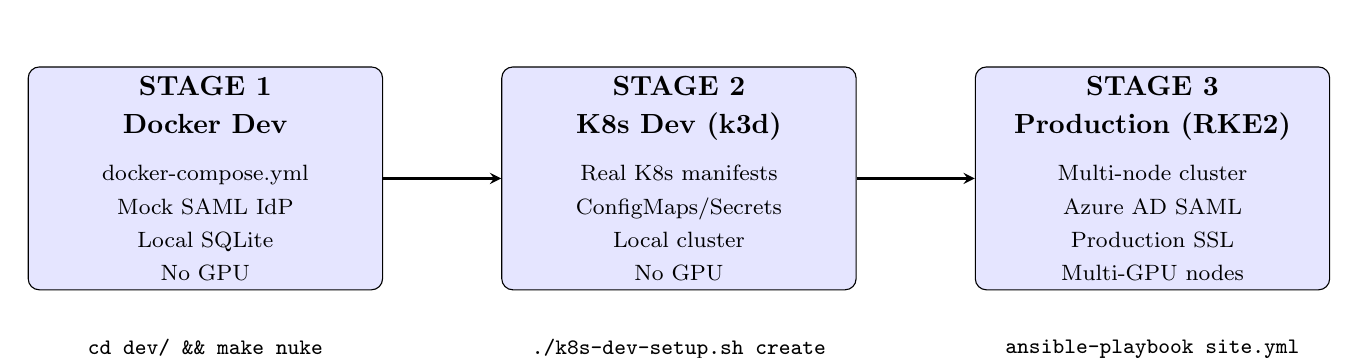
\begin{tikzpicture}[
    node distance=0.3cm,
    stage/.style={rectangle, draw, fill=blue!10, minimum width=4.5cm, minimum height=2.5cm, align=center, rounded corners},
    arrow/.style={->, thick, >=stealth},
    label/.style={font=\small\bfseries}
]

% Stage boxes
\node[stage] (s1) {
    \textbf{STAGE 1}\\[0.2em]
    \textbf{Docker Dev}\\[0.5em]
    \footnotesize docker-compose.yml\\
    \footnotesize Mock SAML IdP\\
    \footnotesize Local SQLite\\
    \footnotesize No GPU
};

\node[stage, right=1.5cm of s1] (s2) {
    \textbf{STAGE 2}\\[0.2em]
    \textbf{K8s Dev (k3d)}\\[0.5em]
    \footnotesize Real K8s manifests\\
    \footnotesize ConfigMaps/Secrets\\
    \footnotesize Local cluster\\
    \footnotesize No GPU
};

\node[stage, right=1.5cm of s2] (s3) {
    \textbf{STAGE 3}\\[0.2em]
    \textbf{Production (RKE2)}\\[0.5em]
    \footnotesize Multi-node cluster\\
    \footnotesize Azure AD SAML\\
    \footnotesize Production SSL\\
    \footnotesize Multi-GPU nodes
};

% Arrows
\draw[arrow] (s1) -- (s2);
\draw[arrow] (s2) -- (s3);

% Commands below
\node[below=0.5cm of s1, font=\ttfamily\footnotesize] {cd dev/ \&\& make nuke};
\node[below=0.5cm of s2, font=\ttfamily\footnotesize] {./k8s-dev-setup.sh create};
\node[below=0.5cm of s3, font=\ttfamily\footnotesize] {ansible-playbook site.yml};

\end{tikzpicture}
\end{center}

\subsection{Quick Start Commands}

\begin{lstlisting}[style=bash]
# STAGE 1: Docker Development (start here)
cd dev/
make nuke          # Complete reset + rebuild

# STAGE 2: Kubernetes Development (after Docker works)
./k8s-dev-setup.sh create

# STAGE 3: Production (after K8s validation)
cd ansible/
ansible-playbook -i inventory.yml playbooks/site.yml
\end{lstlisting}

\begin{infobox}
\textbf{Recommended Workflow:} Always validate changes in Stage 1 (Docker) before promoting to Stage 2 (k3d), and validate in Stage 2 before deploying to Stage 3 (Production).
\end{infobox}

\subsection{Multi-Node Production Architecture}

\begin{center}
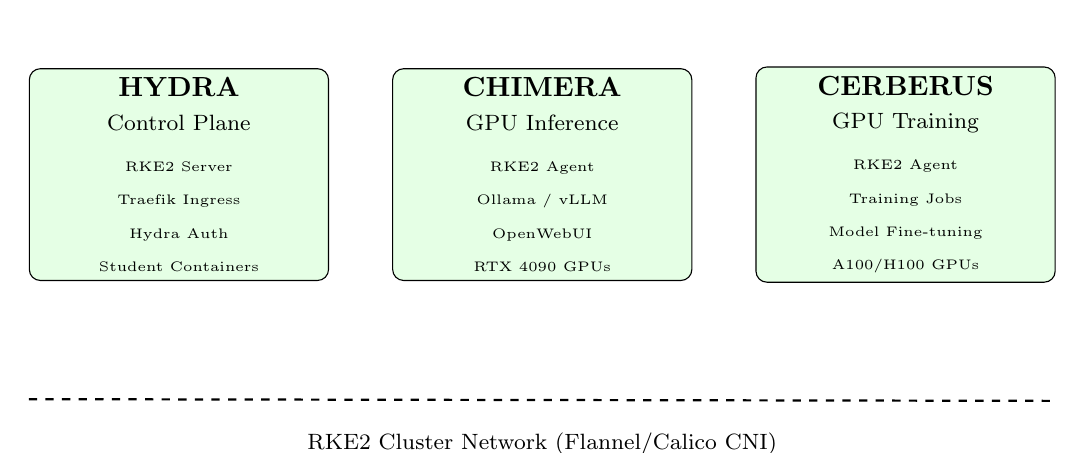
\begin{tikzpicture}[
    node distance=0.8cm,
    server/.style={rectangle, draw, fill=green!10, minimum width=3.8cm, minimum height=2.2cm, align=center, rounded corners},
    label/.style={font=\footnotesize}
]

\node[server] (hydra) {
    \textbf{HYDRA}\\
    \footnotesize Control Plane\\[0.3em]
    \tiny RKE2 Server\\
    \tiny Traefik Ingress\\
    \tiny Hydra Auth\\
    \tiny Student Containers
};

\node[server, right=0.8cm of hydra] (chimera) {
    \textbf{CHIMERA}\\
    \footnotesize GPU Inference\\[0.3em]
    \tiny RKE2 Agent\\
    \tiny Ollama / vLLM\\
    \tiny OpenWebUI\\
    \tiny RTX 4090 GPUs
};

\node[server, right=0.8cm of chimera] (cerberus) {
    \textbf{CERBERUS}\\
    \footnotesize GPU Training\\[0.3em]
    \tiny RKE2 Agent\\
    \tiny Training Jobs\\
    \tiny Model Fine-tuning\\
    \tiny A100/H100 GPUs
};

% Network line
\draw[thick, dashed] ([yshift=-1.5cm]hydra.south west) -- ([yshift=-1.5cm]cerberus.south east);
\node[below=1.8cm of chimera, font=\footnotesize] {RKE2 Cluster Network (Flannel/Calico CNI)};

\end{tikzpicture}
\end{center}

\newpage

\section{Prerequisites}

\subsection{System Requirements}

\begin{table}[H]
\centering
\begin{tabular}{ll}
\toprule
\textbf{Component} & \textbf{Requirement} \\
\midrule
Operating System & Ubuntu 22.04 LTS (recommended) \\
Docker & 24.0+ with Compose V2 \\
RAM & Minimum 8GB (16GB+ recommended) \\
Storage & 100GB+ SSD \\
Network & Static IP, ports 80/443 open \\
\bottomrule
\end{tabular}
\end{table}

\subsection{Required Access}
\begin{itemize}
    \item Azure AD admin access for SAML Enterprise Application setup
    \item DNS control for \texttt{hydra.newpaltz.edu} and subdomains
    \item TLS certificate (Let's Encrypt or institutional cert)
    \item SSH access to the host server
\end{itemize}

\subsection{Software Dependencies}
\begin{lstlisting}[style=bash]
# Install Docker
curl -fsSL https://get.docker.com | sh
sudo usermod -aG docker $USER

# Verify Docker Compose V2
docker compose version
# Should show: Docker Compose version v2.x.x

# Install useful tools
sudo apt install -y git curl jq sqlite3
\end{lstlisting}

\section{Installation Steps}

\subsection{Step 1: Clone Repository}
\begin{lstlisting}[style=bash]
git clone https://github.com/your-org/hydra-saml-auth.git
cd hydra-saml-auth
\end{lstlisting}

\subsection{Step 2: Build Student Container Image}

\begin{lstlisting}[style=bash]
cd student-container
docker build -t hydra-student-container:latest .
cd ..
\end{lstlisting}

\begin{infobox}
This image includes: Ubuntu 22.04, Node.js, Python 3.11+, Java 21, Docker-in-Docker, code-server, and Jupyter.
\end{infobox}

\subsection{Step 3: Configure Environment}

Create \texttt{.env} file in the project root:

\begin{lstlisting}[style=env]
# === Core Settings ===
PORT=6969
BASE_URL=https://hydra.newpaltz.edu
COOKIE_DOMAIN=.newpaltz.edu

# === SAML Configuration ===
METADATA_URL=https://login.microsoftonline.com/YOUR_TENANT/federationmetadata/2007-06/federationmetadata.xml
SAML_SP_ENTITY_ID=hydra-auth
SAML_CALLBACK_URL=https://hydra.newpaltz.edu/auth/callback

# === Database ===
DB_PATH=/app/data/webui.db

# === JWT Settings ===
JWT_TTL_SECONDS=86400
JWT_KEY_ID=hydra-key-1
JWT_PRIVATE_KEY_FILE=/app/certs/jwt-private.pem
JWT_PUBLIC_KEY_FILE=/app/certs/jwt-public.pem

# === Student Containers ===
PUBLIC_STUDENTS_BASE=https://hydra.newpaltz.edu/students

# === OpenWebUI Integration ===
OPENWEBUI_URL=https://gpt.hydra.newpaltz.edu
OPENWEBUI_API_KEY=your-openwebui-api-key

# === n8n Workflow Automation ===
N8N_URL=https://n8n.hydra.newpaltz.edu
N8N_WEBHOOK_URL=https://n8n.hydra.newpaltz.edu/webhook
\end{lstlisting}

\subsection{Step 4: Generate JWT Keys}

\begin{lstlisting}[style=bash]
mkdir -p certs
openssl genrsa -out certs/jwt-private.pem 2048
openssl rsa -in certs/jwt-private.pem -pubout -out certs/jwt-public.pem
\end{lstlisting}

\subsection{Step 5: Configure Azure AD}

\begin{center}
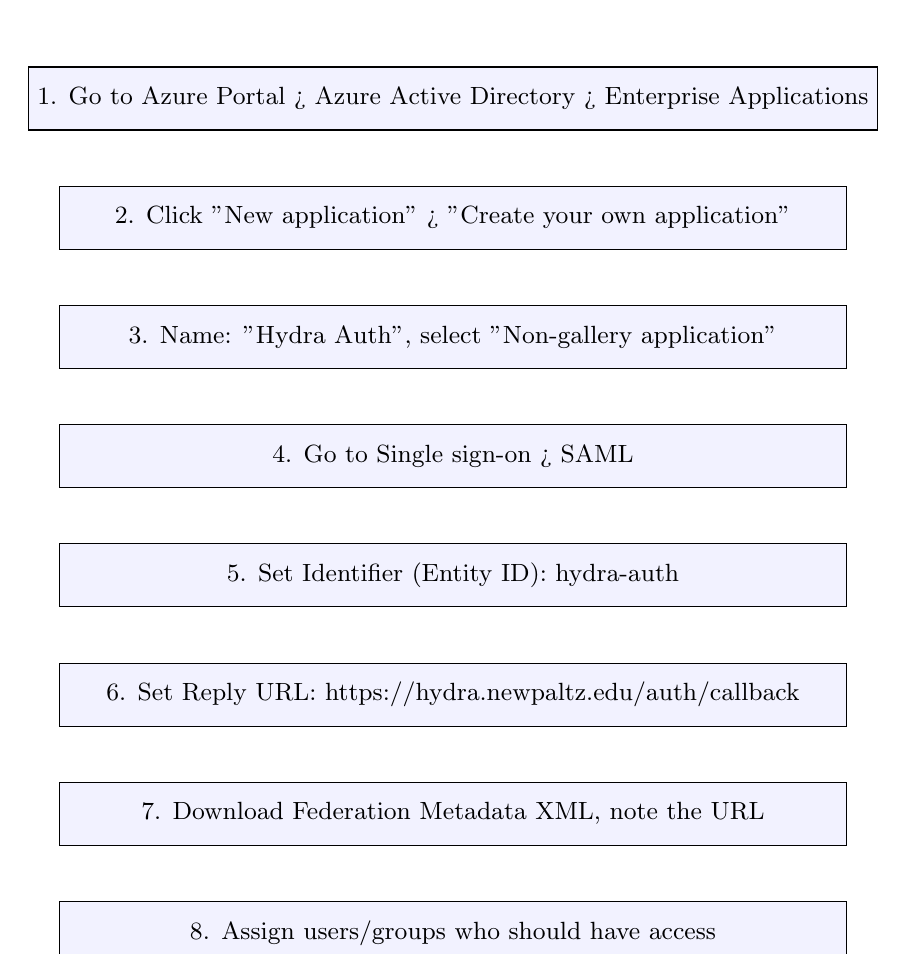
\begin{tikzpicture}[
    node distance=0.7cm,
    stepbox/.style={rectangle, draw, fill=blue!5, minimum width=10cm, minimum height=0.8cm, align=left, font=\small}
]
\node[stepbox] (s1) {1. Go to Azure Portal > Azure Active Directory > Enterprise Applications};
\node[stepbox, below=of s1] (s2) {2. Click "New application" > "Create your own application"};
\node[stepbox, below=of s2] (s3) {3. Name: "Hydra Auth", select "Non-gallery application"};
\node[stepbox, below=of s3] (s4) {4. Go to Single sign-on > SAML};
\node[stepbox, below=of s4] (s5) {5. Set Identifier (Entity ID): hydra-auth};
\node[stepbox, below=of s5] (s6) {6. Set Reply URL: https://hydra.newpaltz.edu/auth/callback};
\node[stepbox, below=of s6] (s7) {7. Download Federation Metadata XML, note the URL};
\node[stepbox, below=of s7] (s8) {8. Assign users/groups who should have access};
\end{tikzpicture}
\end{center}

\begin{warningbox}
\textbf{Critical:} The Entity ID in Azure must \textbf{exactly match} \texttt{SAML\_SP\_ENTITY\_ID} in your \texttt{.env} file.
\end{warningbox}

\subsection{Step 6: Configure Traefik}

Ensure \texttt{docker-compose.yaml} has proper Traefik configuration:

\begin{lstlisting}[style=bash]
# Key Traefik labels for hydra-saml-auth service:
labels:
  - "traefik.enable=true"
  - "traefik.http.routers.hydra.rule=Host(`hydra.newpaltz.edu`)"
  - "traefik.http.routers.hydra.entrypoints=websecure"
  - "traefik.http.routers.hydra.tls=true"
  - "traefik.http.services.hydra.loadbalancer.server.port=6969"
\end{lstlisting}

\subsection{Step 7: Start Services}

\begin{lstlisting}[style=bash]
# Build and start all services
docker compose build
docker compose up -d

# Verify services are running
docker compose ps

# Check logs
docker compose logs -f hydra-saml-auth
\end{lstlisting}

\subsection{Step 8: Verify Installation}

\begin{lstlisting}[style=bash]
# Test HTTPS access
curl -I https://hydra.newpaltz.edu/

# Should redirect to Azure AD login (302 to login.microsoftonline.com)

# Check JWKS endpoint
curl https://hydra.newpaltz.edu/.well-known/jwks.json

# Test OpenWebUI
curl -I https://gpt.hydra.newpaltz.edu/

# Test n8n (if configured)
curl -I https://n8n.hydra.newpaltz.edu/
\end{lstlisting}

\section{Post-Installation Setup}

\subsection{Create Admin User}

After first login via SAML, promote a user to admin:

\begin{lstlisting}[style=bash]
# Access database
sqlite3 /app/data/webui.db

# Find user ID
SELECT id, email, role FROM users WHERE email LIKE '%admin%';

# Set as admin
UPDATE users SET role = 'admin' WHERE email = 'admin@newpaltz.edu';
\end{lstlisting}

\subsection{Test Container Creation}

\begin{enumerate}
    \item Log in to \texttt{https://hydra.newpaltz.edu/dashboard}
    \item Navigate to "Containers" tab
    \item Click "Initialize Container"
    \item Verify VS Code and Jupyter are accessible at:
    \begin{itemize}
        \item \texttt{https://hydra.newpaltz.edu/students/\{username\}/vscode}
        \item \texttt{https://hydra.newpaltz.edu/students/\{username\}/jupyter}
    \end{itemize}
\end{enumerate}

\subsection{Configure Backup Cron}

\begin{lstlisting}[style=bash]
# Add to root crontab
crontab -e

# Daily database backup at 2 AM
0 2 * * * docker exec hydra-saml-auth sqlite3 /app/data/webui.db ".backup '/backups/hydra-$(date +\%Y\%m\%d).db'"

# Weekly cleanup of old backups
0 3 * * 0 find /backups -name "hydra-*.db" -mtime +30 -delete
\end{lstlisting}

\section{Network Architecture}

\subsection{Deployment Diagram}

\begin{center}
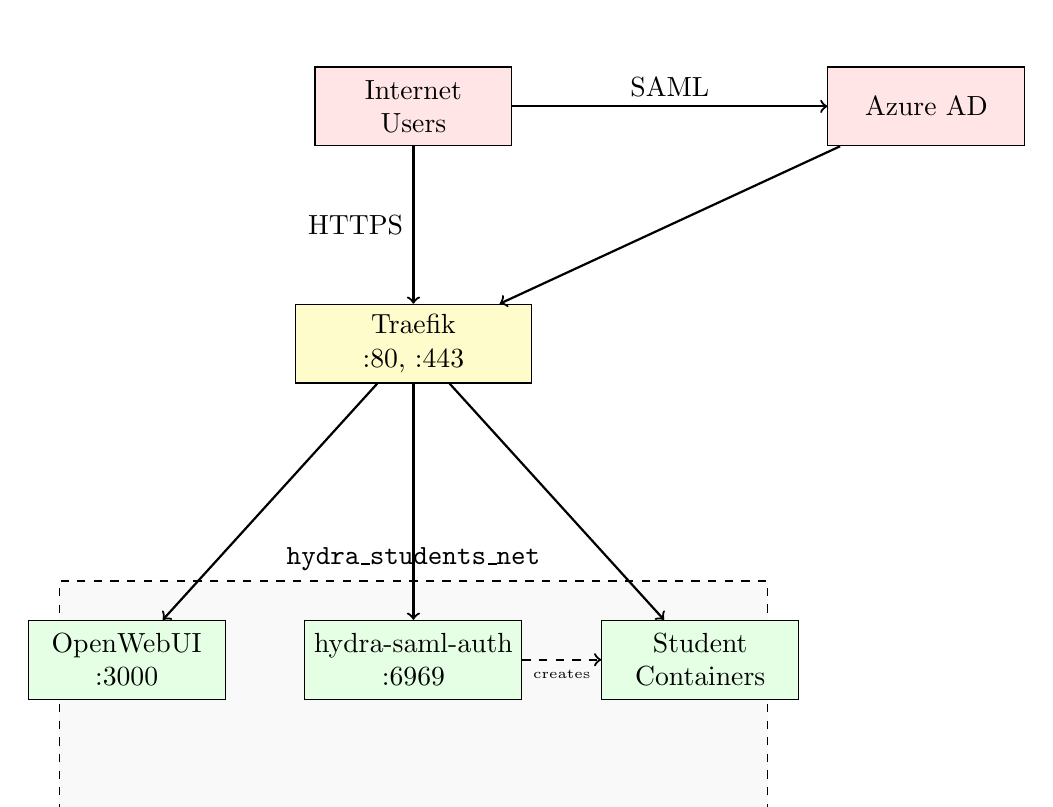
\begin{tikzpicture}[
    node distance=1.2cm,
    ext/.style={rectangle, draw, fill=red!10, minimum width=2.5cm, minimum height=1cm, align=center},
    proxy/.style={rectangle, draw, fill=yellow!20, minimum width=3cm, minimum height=1cm, align=center},
    svc/.style={rectangle, draw, fill=green!10, minimum width=2.5cm, minimum height=1cm, align=center},
    net/.style={rectangle, draw, dashed, fill=gray!5, minimum width=9cm, minimum height=3cm},
    arrow/.style={->, thick}
]

% External
\node[ext] (internet) {Internet\\Users};
\node[ext, right=4cm of internet] (azure) {Azure AD};

% Proxy layer
\node[proxy, below=2cm of internet] (traefik) {Traefik\\:80, :443};

% Internal network
\node[net, below=2.5cm of traefik] (internal) {};
\node[above] at (internal.north) {\texttt{hydra\_students\_net}};

% Services inside network
\node[svc] at ([yshift=0.5cm]internal.center) (hydra) {hydra-saml-auth\\:6969};
\node[svc, left=1cm of hydra] (webui) {OpenWebUI\\:3000};
\node[svc, right=1cm of hydra] (students) {Student\\Containers};

% Arrows
\draw[arrow] (internet) -- node[left] {HTTPS} (traefik);
\draw[arrow] (internet) -- node[above] {SAML} (azure);
\draw[arrow] (azure) -- (traefik);
\draw[arrow] (traefik) -- (hydra);
\draw[arrow] (traefik) -- (webui);
\draw[arrow] (traefik) -- (students);
\draw[arrow, dashed] (hydra) -- node[below, font=\tiny] {creates} (students);

\end{tikzpicture}
\end{center}

\subsection{Port Mapping}

\begin{table}[H]
\centering
\begin{tabular}{llll}
\toprule
\textbf{Service} & \textbf{Internal} & \textbf{External} & \textbf{Protocol} \\
\midrule
Traefik & - & 80, 443 & HTTP/HTTPS \\
hydra-saml-auth & 6969 & via Traefik & HTTP \\
OpenWebUI & 3000 & via Traefik & HTTP \\
Student VS Code & 8443 & /students/\{user\}/vscode & HTTP \\
Student Jupyter & 8888 & /students/\{user\}/jupyter & HTTP \\
\bottomrule
\end{tabular}
\end{table}

\section{Security Configuration}

\subsection{TLS Certificates}

For Let's Encrypt (recommended):
\begin{lstlisting}[style=bash]
# Traefik handles automatic certificate management
# Add to docker-compose.yaml traefik command:
command:
  - "--certificatesresolvers.letsencrypt.acme.email=admin@newpaltz.edu"
  - "--certificatesresolvers.letsencrypt.acme.storage=/letsencrypt/acme.json"
  - "--certificatesresolvers.letsencrypt.acme.httpchallenge.entrypoint=web"
\end{lstlisting}

For institutional certificates:
\begin{lstlisting}[style=bash]
# Mount certificates in Traefik
volumes:
  - ./certs/cert.pem:/certs/cert.pem:ro
  - ./certs/key.pem:/certs/key.pem:ro

# Configure in dynamic config
tls:
  certificates:
    - certFile: /certs/cert.pem
      keyFile: /certs/key.pem
\end{lstlisting}

\subsection{Container Security}

\begin{warningbox}
Student containers run in \textbf{privileged mode} by default to enable Docker-in-Docker. This grants significant access. Consider:
\begin{itemize}
    \item Restricting to trusted users only
    \item Monitoring container activity
    \item Implementing resource quotas
\end{itemize}
\end{warningbox}

\section{Useful Aliases}

Add to \texttt{\textasciitilde/.bashrc}:

\begin{lstlisting}[style=bash]
# ===== HYDRA MANAGEMENT ALIASES =====

# Docker shortcuts
alias dps='docker ps --format "table {{.Names}}\t{{.Status}}\t{{.Ports}}"'
alias dlogs='docker compose logs -f'
alias dexec='docker exec -it'

# Hydra-specific
alias hydra-logs='docker compose logs -f hydra-saml-auth'
alias hydra-restart='docker compose restart hydra-saml-auth'
alias hydra-rebuild='docker compose build hydra-saml-auth && docker compose up -d hydra-saml-auth'

# Student container management
alias students='docker ps --filter "name=student-" --format "table {{.Names}}\t{{.Status}}"'
alias student-logs='docker logs -f'
alias student-shell='docker exec -it'
alias student-stop='docker stop'
alias student-rm='docker rm -f'

# Find student by partial name
findstudent() {
    docker ps --filter "name=student-" --format "{{.Names}}" | grep -i "$1"
}

# Get student container stats
student-stats() {
    docker stats --no-stream --filter "name=student-"
}

# Backup database
backup-db() {
    docker exec hydra-saml-auth sqlite3 /app/data/webui.db ".backup '/backups/hydra-$(date +%Y%m%d-%H%M%S).db'"
    echo "Backup created: hydra-$(date +%Y%m%d-%H%M%S).db"
}

# Quick health check
hydra-health() {
    echo "=== Services ==="
    docker compose ps
    echo ""
    echo "=== Student Containers ==="
    docker ps --filter "name=student-" --format "table {{.Names}}\t{{.Status}}\t{{.RunningFor}}"
    echo ""
    echo "=== Resource Usage ==="
    docker stats --no-stream --format "table {{.Name}}\t{{.CPUPerc}}\t{{.MemUsage}}" | head -10
}
\end{lstlisting}

Apply changes:
\begin{lstlisting}[style=bash]
source ~/.bashrc
\end{lstlisting}

\section{Monitoring}

\subsection{Log Locations}

\begin{table}[H]
\centering
\begin{tabular}{ll}
\toprule
\textbf{Component} & \textbf{Command} \\
\midrule
Main service & \texttt{docker compose logs hydra-saml-auth} \\
Traefik & \texttt{docker compose logs traefik} \\
Student container & \texttt{docker logs student-<username>} \\
All services & \texttt{docker compose logs -f} \\
\bottomrule
\end{tabular}
\end{table}

\subsection{Health Endpoints}

\begin{lstlisting}[style=bash]
# Check main service
curl https://hydra.newpaltz.edu/health

# Check JWKS (JWT verification)
curl https://hydra.newpaltz.edu/.well-known/jwks.json

# Check Traefik dashboard (if enabled)
curl http://localhost:8080/api/overview

# Check OpenWebUI health
curl https://gpt.hydra.newpaltz.edu/health
\end{lstlisting}

\section{Troubleshooting}

\subsection{Common Issues}

\begin{table}[H]
\centering
\begin{tabular}{p{4cm}p{8cm}}
\toprule
\textbf{Issue} & \textbf{Solution} \\
\midrule
SAML login fails & Verify \texttt{METADATA\_URL} accessible, Entity ID matches exactly \\
Student container 404 & Check container on \texttt{hydra\_students\_net}, Traefik running \\
Container won't start & Verify \texttt{hydra-student-container:latest} image built \\
Permission denied & Check Docker socket permissions, user in docker group \\
Database locked & Restart service, check for multiple writers \\
\bottomrule
\end{tabular}
\end{table}

\subsection{Debug Commands}

\begin{lstlisting}[style=bash]
# Check Docker networks
docker network ls
docker network inspect hydra_students_net

# Verify image exists
docker images | grep hydra-student-container

# Check container networking
docker exec student-<user> curl -I http://hydra-saml-auth:6969/

# View Traefik routes
docker exec traefik cat /etc/traefik/traefik.yml
\end{lstlisting}

\section{Upgrade Procedures}

\subsection{Updating the Application}

\begin{lstlisting}[style=bash]
# Pull latest code
git pull origin main

# Rebuild and restart
docker compose build hydra-saml-auth
docker compose up -d hydra-saml-auth

# Verify
docker compose logs -f hydra-saml-auth
\end{lstlisting}

\subsection{Updating Student Container Image}

\begin{lstlisting}[style=bash]
cd student-container
docker build -t hydra-student-container:latest .
\end{lstlisting}

\begin{infobox}
Existing student containers continue using the old image. Students must delete and recreate their container to get the updated image.
\end{infobox}

\section{References}

\subsection{Core Infrastructure}
\begin{itemize}
    \item Docker Documentation: \url{https://docs.docker.com/}
    \item Docker Compose: \url{https://docs.docker.com/compose/}
    \item Docker-in-Docker (DinD): \url{https://docs.docker.com/engine/reference/run/#runtime-privilege-and-linux-capabilities}
    \item Traefik Reverse Proxy: \url{https://doc.traefik.io/traefik/}
    \item Traefik ForwardAuth: \url{https://doc.traefik.io/traefik/middlewares/http/forwardauth/}
    \item Let's Encrypt (TLS Certificates): \url{https://letsencrypt.org/docs/}
\end{itemize}

\subsection{Authentication \& Security}
\begin{itemize}
    \item SAML 2.0 Specification: \url{https://docs.oasis-open.org/security/saml/v2.0/}
    \item Azure AD SAML Setup: \url{https://learn.microsoft.com/en-us/azure/active-directory/develop/single-sign-on-saml-protocol}
    \item Azure AD Enterprise Applications: \url{https://learn.microsoft.com/en-us/azure/active-directory/manage-apps/}
    \item passport-saml (Node.js): \url{https://github.com/node-saml/passport-saml}
    \item JSON Web Tokens (JWT): \url{https://jwt.io/introduction}
    \item JWKS (JSON Web Key Sets): \url{https://auth0.com/docs/secure/tokens/json-web-tokens/json-web-key-sets}
\end{itemize}

\subsection{Development Tools}
\begin{itemize}
    \item code-server (VS Code in Browser): \url{https://coder.com/docs/code-server/latest}
    \item Jupyter Notebook: \url{https://jupyter.org/documentation}
    \item JupyterLab: \url{https://jupyterlab.readthedocs.io/en/stable/}
    \item Node.js: \url{https://nodejs.org/en/docs/}
    \item Python: \url{https://docs.python.org/3/}
    \item OpenJDK: \url{https://openjdk.org/}
\end{itemize}

\subsection{AI \& Automation Services}
\begin{itemize}
    \item OpenWebUI (GPT Interface): \url{https://docs.openwebui.com/}
    \item Ollama (Local LLM Runtime): \url{https://ollama.ai/}
    \item n8n Workflow Automation: \url{https://docs.n8n.io/}
    \item n8n Self-Hosting: \url{https://docs.n8n.io/hosting/}
\end{itemize}

\subsection{Kubernetes (Future Migration)}
\begin{itemize}
    \item RKE2 (Rancher Kubernetes Engine): \url{https://docs.rke2.io/}
    \item Kubernetes Documentation: \url{https://kubernetes.io/docs/}
    \item NVIDIA GPU Operator: \url{https://docs.nvidia.com/datacenter/cloud-native/gpu-operator/}
    \item Longhorn (Distributed Storage): \url{https://longhorn.io/docs/}
\end{itemize}

\subsection{Storage \& Backup}
\begin{itemize}
    \item ZFS on Linux: \url{https://openzfs.github.io/openzfs-docs/}
    \item RAID Levels Explained: \url{https://en.wikipedia.org/wiki/Standard_RAID_levels}
    \item RAID 10 Configuration: \url{https://www.prepressure.com/library/technology/raid}
    \item SQLite Documentation: \url{https://www.sqlite.org/docs.html}
    \item Docker Volumes: \url{https://docs.docker.com/storage/volumes/}
\end{itemize}

\subsection{Game Servers}
\begin{itemize}
    \item Minecraft Server (Java Edition): \url{https://minecraft.wiki/w/Tutorials/Setting_up_a_server}
    \item Minecraft EULA: \url{https://www.minecraft.net/en-us/eula}
    \item itzg/minecraft-server (Docker Image): \url{https://docker-minecraft-server.readthedocs.io/}
\end{itemize}

\subsection{Monitoring \& Logging}
\begin{itemize}
    \item Docker Logs: \url{https://docs.docker.com/config/containers/logging/}
    \item Supervisord (Process Manager): \url{http://supervisord.org/}
    \item htop (Process Viewer): \url{https://htop.dev/}
\end{itemize}

\subsection{SUNY New Paltz Resources}
\begin{itemize}
    \item Hydra Dashboard: \url{https://hydra.newpaltz.edu/dashboard}
    \item OpenWebUI (GPT): \url{https://gpt.hydra.newpaltz.edu/}
    \item SUNY New Paltz ITS: \url{https://www.newpaltz.edu/its/}
\end{itemize}

\begin{successbox}
\textbf{Installation Complete!}

After completing these steps:
\begin{enumerate}
    \item Visit \texttt{https://hydra.newpaltz.edu/login}
    \item Authenticate via Azure AD with your SUNY New Paltz credentials
    \item Navigate to the dashboard
    \item Create a test container to verify the setup
    \item Access VS Code at \texttt{/students/\{username\}/vscode}
    \item Access Jupyter at \texttt{/students/\{username\}/jupyter}
\end{enumerate}

For ongoing management, refer to the \textbf{Hydra Infrastructure Management Guide}.
\end{successbox}

\end{document}
